\documentclass[border=2pt]{standalone}
\usepackage[T1]{fontenc}
\usepackage{mathpazo}
\usepackage{amsmath}
\usepackage{tikz}
\usetikzlibrary{positioning,arrows.meta,fit,calc,backgrounds}
\definecolor{acc}{HTML}{2B6F8A}
\definecolor{accl}{HTML}{E4EFF3}
\definecolor{grl}{HTML}{F2F2F2}
\definecolor{grd}{HTML}{555555}
\begin{document}
\footnotesize\hyphenpenalty=10000\exhyphenpenalty=10000
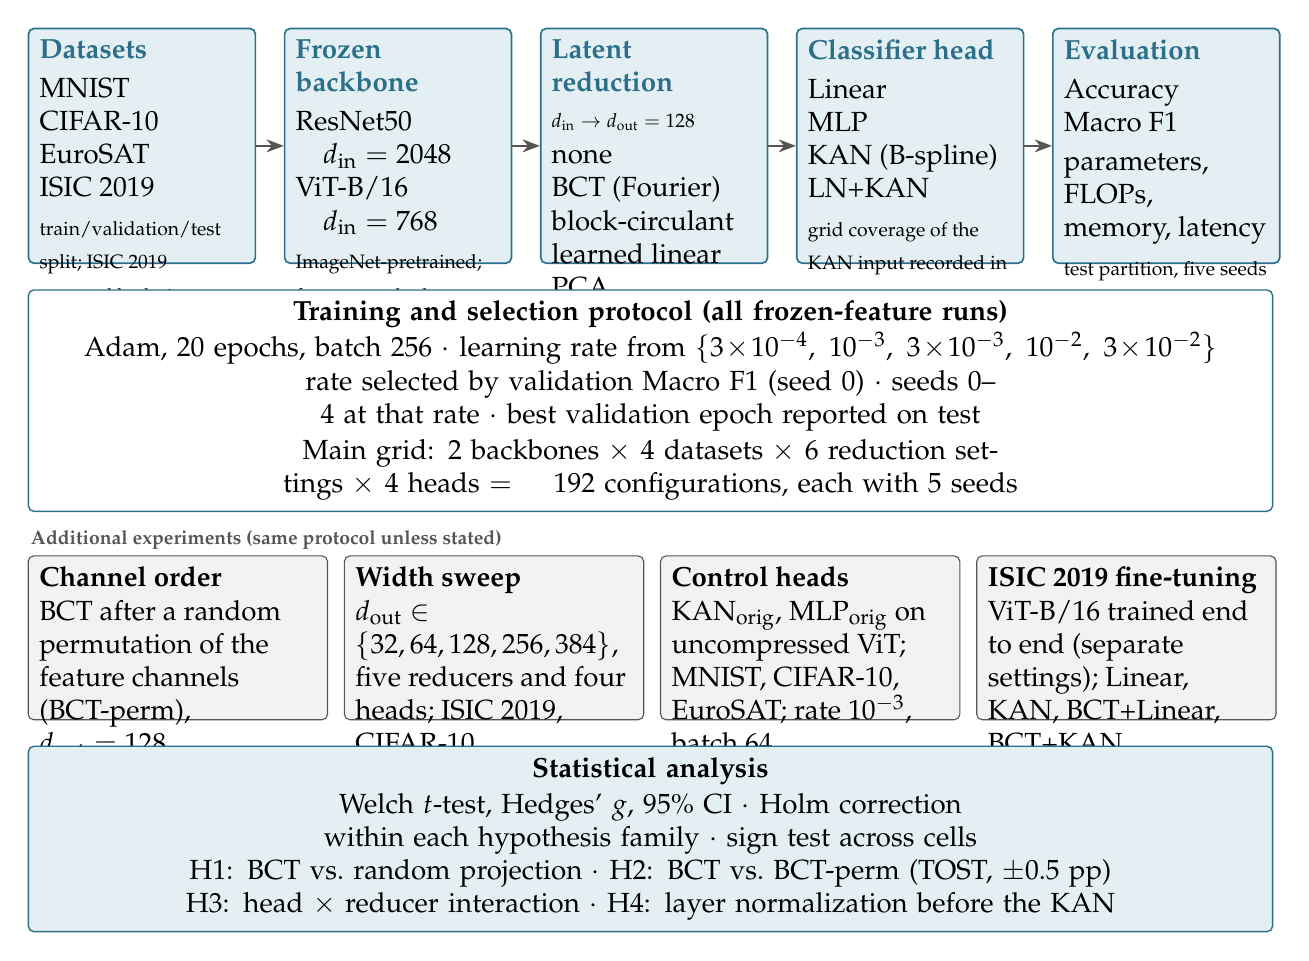
\begin{tikzpicture}[
  stage/.style={draw=acc,line width=0.6pt,fill=accl,rounded corners=2pt,inner sep=4pt,anchor=north,
     execute at begin node={\begin{minipage}[t][2.7cm][t]{2.6cm}\raggedright},
     execute at end node={\end{minipage}}},
  ttl/.style={font=\footnotesize\bfseries,text=acc},
  arr/.style={-{Stealth[length=2.2mm]},line width=0.7pt,draw=grd},
  side/.style={draw=grd,line width=0.4pt,fill=grl,rounded corners=2pt,inner sep=4pt,anchor=north west,
     execute at begin node={\begin{minipage}[t][1.8cm][t]{3.52cm}\raggedright},
     execute at end node={\end{minipage}}},
]
% ---------- main pipeline ----------
\node[stage] (ds) at (0,0) {{\color{acc}\textbf{Datasets}}\\[2pt]
  MNIST\\ CIFAR-10\\ EuroSAT\\ ISIC 2019\\[2pt]
  {\scriptsize train/validation/test split; ISIC 2019 grouped by lesion}};
\node[stage,right=0.35cm of ds.north east,anchor=north west] (bb) {{\color{acc}\textbf{Frozen backbone}}\\[2pt]
  ResNet50\\ \quad $d_{\mathrm{in}}=2048$\\ ViT-B/16\\ \quad $d_{\mathrm{in}}=768$\\[2pt]
  {\scriptsize ImageNet-pretrained; features cached once}};
\node[stage,right=0.35cm of bb.north east,anchor=north west] (rd) {{\color{acc}\textbf{Latent reduction}}\\[1pt]
  {\scriptsize $d_{\mathrm{in}}\rightarrow d_{\mathrm{out}}=128$}\\[1pt]
  none\\ BCT (Fourier)\\ block-circulant\\ learned linear\\ PCA\\ random projection};
\node[stage,right=0.35cm of rd.north east,anchor=north west] (hd) {{\color{acc}\textbf{Classifier head}}\\[2pt]
  Linear\\ MLP\\ KAN (B-spline)\\ LN+KAN\\[2pt]
  {\scriptsize grid coverage of the KAN input recorded in every run}};
\node[stage,right=0.35cm of hd.north east,anchor=north west] (ev) {{\color{acc}\textbf{Evaluation}}\\[2pt]
  Accuracy\\ Macro F1\\[2pt]
  parameters, FLOPs,\\ memory, latency\\[2pt]
  {\scriptsize test partition, five seeds}};
\foreach \a/\b in {ds/bb,bb/rd,rd/hd,hd/ev} \draw[arr] (\a.east) -- (\b.west);
% ---------- protocol strip ----------
\node[draw=acc,line width=0.5pt,rounded corners=2pt,fill=white,align=center,
  text width=15.52cm,inner sep=4pt,anchor=north west] (pr) at ($(ds.south west)+(0,-0.32)$)
  {\textbf{Training and selection protocol (all frozen-feature runs)}\\[1pt]
   Adam, 20 epochs, batch 256 $\cdot$ learning rate from $\{3\!\times\!10^{-4},\ 10^{-3},\ 3\!\times\!10^{-3},\ 10^{-2},\ 3\!\times\!10^{-2}\}$\\
   rate selected by validation Macro F1 (seed 0) $\cdot$ seeds 0--4 at that rate $\cdot$ best validation epoch reported on test\\[1pt]
   Main grid: $2$ backbones $\times$ $4$ datasets $\times$ $6$ reduction settings $\times$ $4$ heads $=192$ configurations, each with 5 seeds};
% ---------- additional experiments ----------
\node[side,anchor=north west] (e1) at ($(pr.south west)+(0,-0.55)$) {\textbf{Channel order}\\
  BCT after a random permutation of the feature channels (BCT-perm), $d_{\mathrm{out}}=128$};
\node[side,right=0.2cm of e1.north east,anchor=north west] (e2) {\textbf{Width sweep}\\
  $d_{\mathrm{out}}\in\{32,64,128,256,384\}$, five reducers and four heads; ISIC 2019, CIFAR-10};
\node[side,right=0.2cm of e2.north east,anchor=north west] (e3) {\textbf{Control heads}\\
  KAN$_{\mathrm{orig}}$, MLP$_{\mathrm{orig}}$ on uncompressed ViT; MNIST, CIFAR-10, EuroSAT; rate $10^{-3}$, batch 64};
\node[side,right=0.2cm of e3.north east,anchor=north west] (e4) {\textbf{ISIC 2019 fine-tuning}\\
  ViT-B/16 trained end to end (separate settings); Linear, KAN, BCT+Linear, BCT+KAN, BCT+LN+KAN};
% ---------- analysis ----------
\node[draw=acc,line width=0.5pt,rounded corners=2pt,fill=accl,align=center,
  text width=15.52cm,inner sep=4pt,anchor=north west] (an) at ($(e1.south west)+(0,-0.32)$)
  {\textbf{Statistical analysis}\\[1pt]
   Welch $t$-test, Hedges' $g$, 95\% CI $\cdot$ Holm correction within each hypothesis family $\cdot$ sign test across cells\\
   H1: BCT vs.\ random projection $\cdot$ H2: BCT vs.\ BCT-perm (TOST, $\pm0.5$ pp)\\ H3: head $\times$ reducer interaction $\cdot$ H4: layer normalization before the KAN};
\node[font=\scriptsize\bfseries,text=grd,anchor=south west,inner sep=1pt] at ($(e1.north west)+(0,0.03)$) {Additional experiments (same protocol unless stated)};
\end{tikzpicture}
\end{document}
